\documentclass[a4paper]{article}
\usepackage{booktabs}
\usepackage{array}
\usepackage{wrapfig}
\usepackage{multirow}
\usepackage{tabularx}
\usepackage{graphicx}
\usepackage{authblk}
\usepackage{pgf, tikz}
\usetikzlibrary{positioning}
\usetikzlibrary{decorations.pathreplacing}
\usepackage[margin=0.375cm]{subcaption}
\usepackage{footnote}
\usepackage[symbol*]{footmisc}
\renewcommand*{\thefootnote}{\arabic{footnote}}
\makesavenoteenv{figure}
\usepackage{amsmath}
\usepackage{amsthm}
\usepackage{amssymb}
\usepackage{mdframed}
\usepackage{csquotes}
\usepackage{polyglossia}
\usepackage{pifont}
\newcommand{\cmark}{\ding{51}}%
\newcommand{\xmark}{\ding{55}}%
\setdefaultlanguage{english}
\usepackage[style=alphabetic,minalphanames=3,maxbibnames=99]{biblatex}
\usepackage{hyperref}
\usepackage{cleveref}
\crefname{section}{\S}{\S\S}
\Crefname{section}{\S}{\S\S}

\def\bitcoinA{%
  \leavevmode
  \vtop{\offinterlineskip %\bfseries
    \setbox0=\hbox{B}%
    \setbox2=\hbox to\wd0{\hfil\hskip-.03em
    \vrule height .3ex width .15ex\hskip .08em
    \vrule height .3ex width .15ex\hfil}
    \vbox{\copy2\box0}\box2}}

\addbibresource{references.bib}

\usetikzlibrary{arrows, automata}

\def\bitcoinA{%
  \leavevmode
  \vtop{\offinterlineskip %\bfseries
    \setbox0=\hbox{B}%
    \setbox2=\hbox to\wd0{\hfil\hskip-.03em
    \vrule height .3ex width .15ex\hskip .08em
    \vrule height .3ex width .15ex\hfil}
    \vbox{\copy2\box0}\box2}}

% reduce page count
\addtolength{\oddsidemargin}{-.875in}
\addtolength{\evensidemargin}{-.875in}
\addtolength{\textwidth}{1.75in}
\addtolength{\topmargin}{-.875in}
\addtolength{\textheight}{1.75in}

%\setlength{\belowcaptionskip}{-10pt}

\begin{document}
\title{WabiSabi: Centrally Coordinated CoinJoins with Variable Amounts}
\author[1]{Ádám Ficsór}
\author[1]{Yuval Kogman}
\author[1]{Lucas Ontivero}
\author[2]{István András Seres}
\affil[1]{zkSNACKs}
\affil[2]{Eötvös Loránd University}
\date{}
\maketitle

\begin{abstract}
Bitcoin transfers value on a public ledger of transactions anyone can verify. Coin ownership is defined in terms of public keys.
Despite potential use for private transfers, research has shown that users' activity can often be traced in practice. Businesses have been built on dragnet surveillance of Bitcoin users because of this lack of strong privacy, which harms its fungibility, a basic property of functional money.

Although the public nature of this design lacks strong guarantees for privacy, it does not rule it out.
A number of methods have been proposed to strengthen privacy. Among these is CoinJoin, an approach based on multiparty transactions that can introduce ambiguity and break common assumptions that underlie heuristics used for deanonymization.
Existing implementations of CoinJoin have several limitations which may partly explain the lack of their widespread adoption.

This work introduces \emph{WabiSabi}\footnote{The Japanese concept \emph{wabi-sabi} is an aesthetic world view which among other things emphasizes acceptance of imperfections, in our case Bitcoin's challenges for privacy, and an appreciation for simplicity and economy.}, a new protocol for centrally coordinated CoinJoin implementations utilizing keyed verification anonymous credentials and homomorphic value commitments. This improves earlier approaches which utilize blind signatures in both privacy and flexibility, enabling novel use cases and reduced overhead.
\end{abstract}

\section{Introduction}
Bitcoin transactions transfer funds by consuming unspent outputs of previous transactions as inputs to create new outputs~\cite{nakamoto2009bitcoin}. The protocol rules enforced by the network ensure that transactions do not arbitrarily inflate the money supply and that outputs are spent at most once. While some newer cryptocurrencies use more sophisticated approaches to define such rules, in Bitcoin the amounts, as well as the specific outputs being spent, are broadcast in the clear as part of the transaction. This presents significant challenges to transacting privately\footnote{In this work we restrict the discussion of Bitcoin privacy to that of public ledger transactions, but there are other considerations especially at the network layer. For a more comprehensive discussion see \url{https://en.bitcoin.it/wiki/Privacy}.} as shown already in some of the earliest academic studies of Bitcoin~\cite{reid2013analysis,ron2013quantitative,androulaki2013evaluating,ober2013structure,moeser2013inquiry,meiklejohn2013fistful}.

A fundamental requirement for electronic money is double-spending prevention, and Bitcoin's main innovation was preventing double-spending and illegal inflation without relying on a trusted authority, thereby disintermediating transactions. This is in contrast to online e-cash schemes where a server authorizes transactions or offline schemes where the identity of the double spender is revealed allowing the authority to intervene after the fact. Bitcoin's relative success in comparison suggests that the lack of trusted third parties factored more strongly in its adoption than the comparatively stronger privacy guarantees provided by the (possibly revocable) transaction  anonymity traditionally associated with e-cash~\cite{davida1997anonymity}.

These shortcomings in privacy affect Bitcoin users, both individuals and organizations, leaving casual users especially vulnerable since power to surveil and resist surveillance is unevenly distributed~\cite{rogaway2015moral}. Even without address reuse, which is widespread~\cite{gaihre2018bitcoin}, transactions still reveal some information. This makes clustering of outputs according to heuristics practical~\cite{harrigan2016unreasonable}, with wallets of some well-known entities generally considered public knowledge. Exchanges complying KYC/AML requirements additionally must collect and safeguard information that links transactions to personally-identifying information.

The conditions for spending an output are specified in its \texttt{scriptPubKey}, typically requiring that the spending transaction be signed by a particular key. The signatures authorizing a transaction usually commit to the transaction in its entirety, making it possible for mutually distrusting parties to jointly create transactions without risking misallocation of funds: participants will only sign a proposed transaction after confirming that their desired outputs are included and the transaction is only valid when all parties have signed.

\subsection{Chaumian CoinJoin}

Chaumian CoinJoin~\cite{mizrahi2013blind,maxwell2013coinjoin,zerolink} is a privacy-enhancing technique that uses the atomicity of transactions and Chaumian blind signatures~\cite{chaum1983blind} to construct collaborative Bitcoin transactions, also known as CoinJoins. Participants connect to a server, known as the \emph{coordinator}, and submit their inputs and outputs using different anonymity network identities. That alone would provide anonymity but since outputs are unconstrained it's not robust against malicious users who may disrupt the protocol by claiming more than their fair share in the transaction outputs. To mitigate this the coordinator provides blind signatures representing units of standard denominations in response to submitted inputs. Clients unblind and submit the output with valid signature, which allows them to verify that an output registration is authorized without being able to link it to the corresponding inputs.

The use of standard denominations in the resulting CoinJoin transaction obscures the relationship between individual inputs and outputs, making the origins of each output ambiguous. Unfortunately, standard denominations limit the use of privacy-enhanced outputs for payments of arbitrary amounts and result in a change output which maintains a link to the non-private input.

\subsection{Our Contribution}

We present WabiSabi, a generalization of Chaumian CoinJoin based on a keyed-verification anonymous credentials (KVAC) scheme~\cite{chase2019signal}. The use of KVACs replaces blind signatures' standard denominations with homomorphic amount commitments, similar to Confidential Transactions~\cite{maxwell2016confidential}, where the sum of any participant's outputs does not exceed that of their inputs while hiding the underlying values from the coordinator. In addition to being more flexible, this improves privacy compared to blind signatures and standard denominations since smaller inputs can be combined and change outputs created with the same unlinkability guarantees as those of standard denominations when using blind signatures\footnote{Note that the cleartext amounts appearing in the final transaction might still link individual inputs and outputs.}. WabiSabi builds on a successfully deployed and proven approach, aiming to reduce barriers to further adoption~\cite{dingledine2006anonymity} by removing restrictions and strengthening unlinkability.

WabiSabi can be instantiated to construct a variety of CoinJoin transaction structures that depart from the standard output denomination convention, as in SharedCoin\footnote{See: \url{https://github.com/sharedcoin/Sharedcoin}} and CashFusion\footnote{See: \url{https://github.com/cashshuffle/spec}} style transactions and Knapsack~\cite{maurer2017anonymous} mixing. Payments from CoinJoin transactions are possible which enhances sender privacy, as are payments within CoinJoin transactions, improving privacy for both sender and receiver and potentially hiding the payment amount. Additionally, restrictions on the consolidation of inputs can be removed, and there are opportunities for reducing unmixed change, relaxing minimum required denominations, and improved block space efficiency compared to what is possible with blind signatures.

The rest of this paper is organized as follows. We present necessary background knowledge about privacy issues of Bitcoin in~\cref{sec:background}. In \cref{sec:preliminaries} we provide some preliminaries on our applied cryptographic building blocks. We introduce our system model in~\cref{sec:systemmodel}. In \cref{sec:overview} we introduce our protocol, WabiSabi, at a high-level, while in \cref{sec:details} we describe in-depth the cryptographic details of WabiSabi. In \cref{sec:securitayandprivacy} we argue about the security and privacy of WabiSabi. A report on our preliminary implementation is provided in \cref{sec:performanceanalysis}. We review related work in \cref{sec:relatedwork}. We outline ongoing and future work in~\cref{sec:futuredirections}. Finally, we conclude our paper in \cref{sec:conclusion}.

\section{Background and Motivation} \label{sec:background}

In this section, we provide an introduction to Bitcoin privacy issues and proposals to enhance transaction privacy. We detail current limitations of Bitcoin privacy-enhancing tools and motivate our work.

\subsection{Privacy issues and CoinJoin transactions}

Bitcoin is a pseudonymous cryptocurrency~\cite{nakamoto2009bitcoin}: coins are associated with so called addresses, which encode the spending conditions of the coin (their \texttt{scriptPubKey}). Bitcoin transactions spend coins as inputs and create new coins output in place of the spent ones. The Bitcoin protocol mandates the rules of a valid transaction (no double-spending, valid signatures, etc.), which is verified by all nodes of the network. Since every transaction is recorded in a public ledger, the flow of money is traceable. Several idioms of use allow one to cluster addresses likely to be controlled by the same user. Many heuristics were devised in previous work~\cite{meiklejohn2013fistful,androulaki2013evaluating,reid2013analysis,ron2013quantitative}. The most commonly used heuristic to cluster Bitcoin addresses is the \emph{common input ownership heuristic}. It states that in any Bitcoin transaction, all the inputs are likely controlled by the same user. This heuristic already facilitates a fine-grained clustering of Bitcoin addresses, with alarming accuracy\cite{nick2015data}.

\begin{figure}
    \centering
\begin{tikzpicture}[mynode/.style={draw, anchor=center}]

% tableu qualitative color scheme
\definecolor{c1}{HTML}{4e79a7}
\definecolor{c2}{HTML}{f28e2b}
\definecolor{c3}{HTML}{59a14f} % green, use for mixed
\definecolor{c4}{HTML}{e15759}
\definecolor{c5}{HTML}{76b7b2}
\definecolor{c6}{HTML}{edc948}
\definecolor{c7}{HTML}{b07aa1}
\definecolor{c8}{HTML}{ff9da7}

\node [mynode,fill=c4,label={\textbf{Inputs}}] at (0,0)  {\textbf{$1.1$\bitcoinA{}}};
\node [mynode,fill=c2] at (0,-1)  {\textbf{$1.3$\bitcoinA{}}};
\node [mynode,fill=c1] at (0,-2)  {\textbf{$1.5$\bitcoinA{}}};
\node [mynode,,fill=c3,label={\textbf{Outputs}}] at (2,0) (a) {\textbf{$1.0$\bitcoinA{}}};
\node [mynode,fill=c3] at (2,-1)  {\textbf{$1.0$\bitcoinA{}}};
\node [mynode,fill=c3] at (2,-2)  {\textbf{$1.0$\bitcoinA{}}};
%% here comes the change outputs
\node [mynode,fill=c4] at (2,-3)   {\textbf{$0.1$\bitcoinA{}}};
\node [mynode,fill=c2] at (2,-4)  {\textbf{$0.3$\bitcoinA{}}};
\node [mynode,fill=c1] at (2,-5) (c) {\textbf{$0.5$\bitcoinA{}}};
\draw [decoration={brace}, decorate] (3,0.4) -- node [xshift=12ex] {\textbf{``Mixed" outputs}} (3,-2.4);
\draw [decoration={brace}, decorate] (3,-2.6) -- node [xshift=12ex] {\textbf{Change outputs}} (3,-5.4);
\draw (-0.8,1) rectangle (2.8,-5.8);
\node[label={\textbf{CoinJoin tx}}] at (1.2,0.9) {};
%%first postmix transaction
\node [mynode,fill=c3,label={\textbf{Input}}] at (8,0) (B)  {\textbf{$1.0$\bitcoinA{}}};
%\node [above=2mm of a] {label1};
\draw[->]
  (a) edge (B);
\node [mynode,fill=c5,label={\textbf{Outputs}}] at (10,0) (C)  {\textbf{$0.8$\bitcoinA{}}};
\node [mynode,fill=c6] at (10,-1) (C)  {\textbf{$0.2$\bitcoinA{}}};
\draw (7.2,1) rectangle (10.8,-1.8);
\node[label={\textbf{Non-attributable tx}}] at (9.1,0.9) {};
%%second postmix transaction
\node [mynode,fill=c1,label={\textbf{Input}}] at (8,-5) (D)  {\textbf{$0.5$\bitcoinA{}}};
%\node [above=2mm of a] {label1};
\draw[->]
  (c) edge (D);
\node [mynode,fill=c7,label={\textbf{Outputs}}] at (10,-4) (D)  {\textbf{$0.2$\bitcoinA{}}};
\node [mynode,fill=c8] at (10,-5) (D)  {\textbf{$0.3$\bitcoinA{}}};
\draw (7.2,-3) rectangle (10.8,-5.8);
\node[label={\textbf{Attributable tx}}] at (9.1,-3.1) {};
\end{tikzpicture}
\caption{A simple CoinJoin transaction and two post-mix transactions. Privacy-enhanced outputs are colored green. Each of them improved their $k$-anonymity ($k=3$). Change outputs have the color of their corresponding inputs. Arrows indicate which transaction output has been spent by the referencing transaction input. The payer of the first post-mix transaction is non-attributable. However, the payer of the second post-mix transaction is easily linkable to the third input of the CoinJoin transaction, since the post-mix transaction spends a change output of the CoinJoin transaction. Coins are only represented by their BTC (\bitcoinA{}) value. For simplicity, transaction fees are omitted.}
\label{fig:simplecoinjoin}
\end{figure}

CoinJoin transactions aim to contradict to the common ownership heuristic, because multiple users collaboratively create the transaction. There are several types of privacy-enhancing techniques in Bitcoin, e.g. PayJoin\footnote{See: \url{https://en.bitcoin.it/wiki/PayJoin}}, CoinSwap~\cite{belcher2020design}. However, in this work, we solely focus on CoinJoins. In an equal-amount CoinJoin transaction (see \cref{fig:simplecoinjoin}) each user contributes at least one input and receives at least one output with the same amount as the other users. Assuming the output types are uniform individual outputs differ only in the keys associated with them, which are indistinguishable from uniformly random data. Consequentially it is not possible to link inputs to specific mixed outputs. The privacy of such outputs can be modeled using $k$-anonymity~\cite{sweeney2002k} with amounts and script types as quasi-identifiers, but this analysis becomes rather complicated in a broader context than that of a single transaction in isolation because the graph structure can reveal additional information.

\subsubsection{Wasabi's ZeroLink Protocol}

Several CoinJoin protocols have been implemented and many more proposed, with varying privacy and trust models. For an overview see~\cref{sec:relatedwork}. ZeroLink~\cite{zerolink} is one such protocol implemented by Wasabi, the most popular Chaumian CoinJoin implementation for Bitcoin. Although the coordinator must be trusted to ensure availability, but no trust is required with regards to safeguarding users' funds or keeping mapping between inputs and outputs private. The protocol breaks down into three main phases:

\begin{description}
 \item[Input Registration] Users register their inputs along with proofs (digital signatures) that they own those inputs. Additionally, users provide their change outputs and blinded outputs to the coordinator. The coordinator blindly signs the requested blinded output.
 \item[Output Registration] Users unblind their signatures received from the coordinator and register their outputs. We note that input and output registrations are completed using different network identifiers (Tor circuits) to ensure network-level privacy as well.
 \item[Signing] Users receive the unsigned CoinJoin transaction from the coordinator. If it contains their requested inputs and outputs, users sign the transaction and send back to the coordinator their signature(s). If all signatures are received, the coordinator broadcasts the final, signed CoinJoin transaction.
\end{description}

\subsection{Limitations of Wasabi}\label{sec:limitations}
In this work, we aim to improve on the ZeroLink protocol as implemented in Wasabi. We identify several privacy shortcomings and inefficiencies of Wasabi CoinJoins. Specifically, we are interested in quantifying block-space and other inefficiencies stemming from the imposed minimum denomination. These metrics comparing Wasabi, Samourai's Whirlpool\footnote{See: \url{https://www.samouraiwallet.com/whirlpool}}, and other apparent CoinJoin transactions are provided. The ``Other'' category includes JoinMarket\footnote{See: \url{https://github. com/JoinMarket-Org/joinmarket}}, but also has an inherent false positive error given these transactions are identified heuristically. We collected every equal output CoinJoin-like transactions from the Bitcoin blockchain till 2020 May 22nd. Wasabi and Samourai CoinJoin transactions are trivial to detect. A transaction that has more than $10$ equal amount outputs are surely Wasabi CoinJoins, while a Samourai CoinJoin transaction has the same structure, with $5$ equal amount outputs of a fixed size, $3$ inputs of exactly the same amount, while fees are paid by $2$ inputs of a slightly higher amount which are direct descendants of a so called ``tx0'', a transaction that prepares outputs for mixing and pays the coordination fees. However, other CoinJoin transactions, e.g. JoinMarket, are more difficult to identify~\cite{moeser2017anonymous}. Heuristically, we deem every transaction being in the ``Other'' CoinJoin transaction category if they simultaneously satisfy the following conditions:

\begin{itemize}
    \item There are at least two equal amount outputs. We refer to the number of equal amount outputs as the size of the anonymity set.
    \item The number of distinct public keys of the inputs is at least the size of the anonymity set.
    \item The number of distinct public keys of the outputs is at least the size of the anonymity set.
\end{itemize}

The first requirement ensures that transactions in the ``Other'' category are indeed privacy-enhancing transactions. The second and third requirements filter out batching and exchange deposit/withdraw transactions. However, we acknowledge that this heuristic might incur a few false positives as well as false negatives.

A cross platform tool for the reproducible analysis of Bitcoin privacy-enhancing transactions was developed and released~\footnote{See: \url{https://github.com/nopara73/Dumplings}} to facilitate this as well as further research. We report our findings in more detail.

\subsubsection{Denominations}

Due to the nature of blind signatures, mixed outputs of Wasabi CoinJoins are restricted to a fixed set of multiples of a base denomination\footnote{Approximately $0.1$\bitcoinA{}}. This creates friction when sending or receiving arbitrary amounts of Bitcoin, as using fixed denomination generally creates change, both when mixing and when spending mixed outputs. Non-mixed change outputs in a CoinJoin are almost always linkable to their corresponding inputs. Therefore, every Bitcoin privacy-enhancing tool should aim to minimize the number of unmixed change outputs.

We define \emph{CoinJoin inefficiency} as the fraction of non-mixed change outputs in a CoinJoin transaction. In~\cref{fig:cjinefficiency}, we observe the large amount of non-mixed outputs of essentially all Bitcoin privacy-enhancing tools. Samourai has the lowest CoinJoin inefficency, since it always applies $5$ equal amount of inputs and outputs. We note a sharp decline of CoinJoin inefficiency in Wasabi CoinJoins around January 2019 due to the introduction of multiples of the base denomination.

\begin{figure}[h!]
    \centering
    \includegraphics[scale=0.4]{Figures/CJInefficiency.pdf}
    \caption{CoinJoin inefficiency of various privacy-focused Bitcoin wallets. We define CoinJoin inefficiency to be the fraction of non-mixed change outputs and the total number of outputs in a CoinJoin transaction. A higher value indicates more block space required to mix a given volume of Bitcoin. All CoinJoin implementations tools produce a significant amount of ``toxic change" due to the requirement of mixed outputs being uniform, either directly from CoinJoin transactions or in Samourai's case from antecessor transactions that prepare outputs for mixing.}
    \label{fig:cjinefficiency}
\end{figure}

\subsubsection{Minimum denomination}

In order to participate in a CoinJoin, a user's combined input amount must be greater or equal to the base denomination.\footnote{The observed base denominations in Wasabi's CoinJoins are usually slightly higher than the announced, agreed upon base denomination. Thus, participants sometimes get back slightly more value in the CoinJoins than they put in.} We observe, that considerable portion of CoinJoin inputs are less than this minimum denomination, see \cref{fig:minimumdenomination}.

\begin{figure}%[ht!]
\centering
\begin{minipage}{.45\textwidth}
    \centering
    \includegraphics[width=\linewidth]{Figures/SmallValueInputsWasabi.pdf}
    \caption{Fraction of inputs with value smaller than the minimum denomination in Wasabi CoinJoin transactions.}
    \label{fig:minimumdenomination}
\end{minipage}
\hspace{6pt}
\begin{minipage}{.45\textwidth}
    \centering
    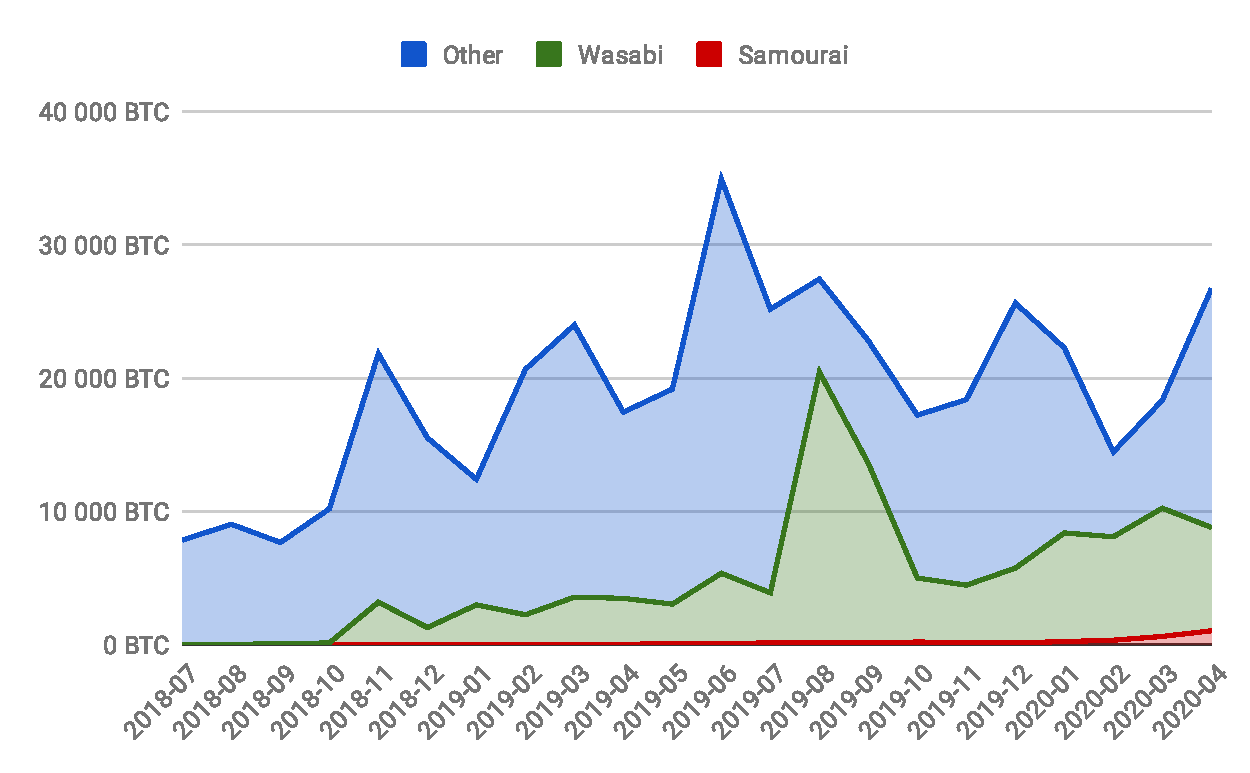
\includegraphics[width=0.95\linewidth]{Figures/freshBitcoins.pdf}
    \caption{Volume of unmixed coins entering to various CoinJoin schemes. Wasabi is the most popular Chaumian CoinJoin implementation.}
    \label{fig:freshBitcoins}
\end{minipage}
\end{figure}

Even when users are able to provide several smaller value inputs with a total value greater than the minimum denomination, the coordinator learns that those inputs belong to the same user. In an ideal mixing protocol, the coordinator should not obtain more information by coordinating the CoinJoin transaction than what the publicly available blockchain data reveals. This information removes many degrees of freedom when assigning non-derived sub-transactions~\cite{maurer2017anonymous} or link probability~\cite{laurentmt2015bitcoin}, reducing intrinsic ambiguity as well as the computational cost when evaluating potential links.

Furthermore, if users consolidate coins in an additional transaction before participating in a CoinJoin, then this link is revealed publicly based on the common input ownership heuristic~\cite{meiklejohn2013fistful}.

\subsubsection{Varying denominations} Since users pay mining and coordination fees the base denomination is gradually reduced between rounds of consecutive CoinJoins. This makes it possible for users to mix several times without providing additional inputs. In Wasabi remixed coins are not required to pay coordination fees if they are very close to the base denomination, which introduces a perverse incentive to minimize coordination fees by remixing in quick succession in order, resulting in a smaller anonymity set than with time-staggered remixes.

\subsubsection{Block-space efficiency}

The rigidity of the current transaction structure, i.e. fixed denominations, constrains users' unspent transaction output set structure as well. These limitations force users to consolidate their coins (see \cref{fig:postmixmerging}) and create additional intermediate outputs with constrained amounts when interspersing CoinJoin transactions with transactions that send or receive value.

\begin{figure}%[ht!]
\centering
\begin{minipage}{.45\textwidth}
    \centering
    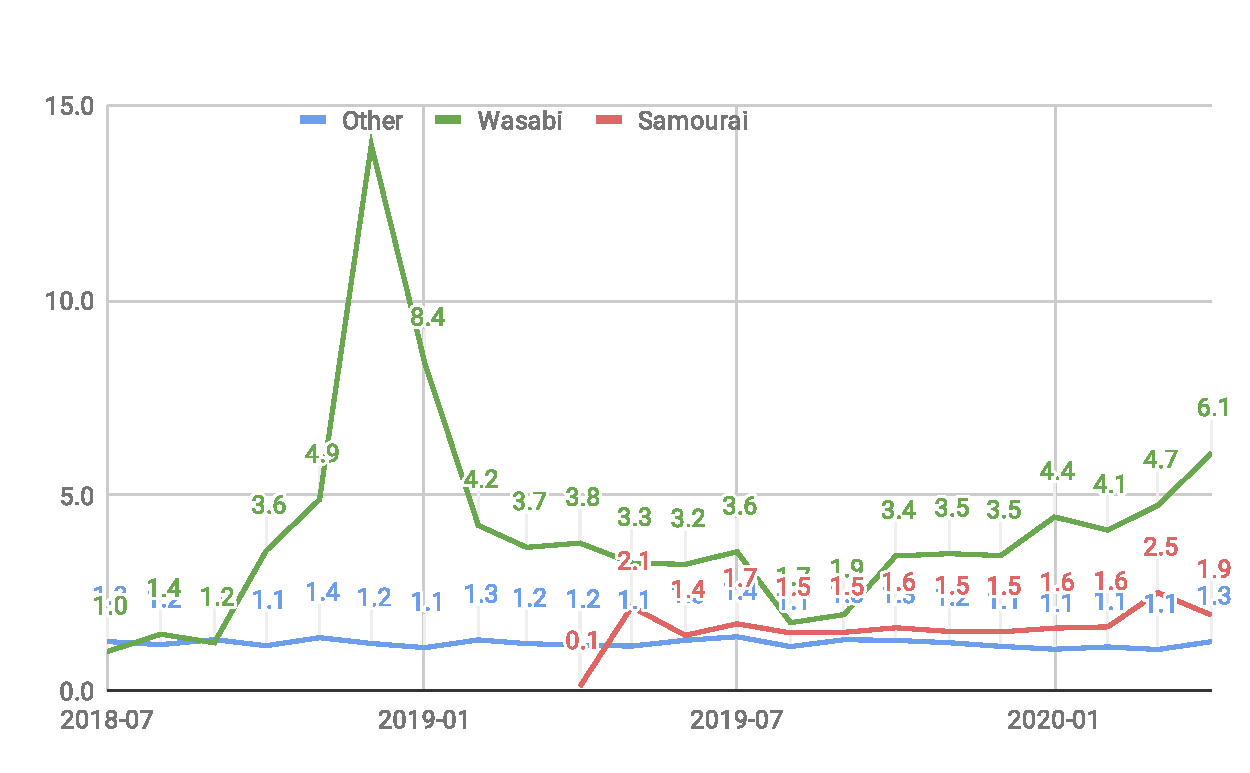
\includegraphics[width=\linewidth]{Figures/avgRemixCount.pdf}
    \caption{Average remix count of various Bitcoin privacy-enhancing tools. Remixing increases user privacy at the expense of block-space efficiency. }
    \label{fig:remixcount}
\end{minipage}
\hspace{6pt}
\begin{minipage}{.45\textwidth}
    \centering
    \includegraphics[width=0.95\linewidth]{Figures/postMixInputMerging.pdf}
    \caption{Average number of inputs from the first post-mix transactions in various CoinJoin schemes. The large figures for other CoinJoin-like transactions suggests false positives in our identification.}
    \label{fig:postmixmerging}
\end{minipage}
\end{figure}

\subsubsection{Lack of privacy-enhanced payments} Currently, Wasabi supports neither payments from a CoinJoin, nor payments in a CoinJoin. Payments from a CoinJoin would protect sender privacy and improve efficiency by requiring fewer intermediate outputs. Payments within a CoinJoin would protect both sender and receiver privacy, as well as undermine clustering heuristics since they are analogous to PayJoins. It would also improve privacy by introducing degrees of freedom in the interpretation of CoinJoins.




\section{Preliminaries}\label{sec:preliminaries}

Hereby we give an informal and high-level description of applied cryptographic primitives. In the following, the security parameter is denoted as $\lambda$.

\subsection{Commitment schemes}
A commitment scheme allows one to commit to a chosen message while preventing them from changing the message after publishing the commitment. Secure commitments hide the chosen message until they are opened. We assume Pedersen commitments throughout this work.

\begin{description}

\item[$\mathsf{Commit}(m,r)\mapsto{}\mathcal{C}$:] generate a commitment $\mathcal{C}$ to message $m$ using randomness $r$.

\item[$\mathsf{OpenCom}(\mathcal{C},m,r)\mapsto{}\{\mathit{True},\mathit{False}\}$:] verify the correctness of the opening of a commitment by checking $\mathcal{C}\stackrel{?}{=}\mathsf{Commit}(m,r)$. If equality holds the algorithm outputs $\mathit{True}$, otherwise $\mathit{False}$.

\end{description}

\subsection{MAC}
A message authentication code (MAC) ensures the integrity of a message and consists of the following three probabilistic polynomial-time algorithms:

\begin{description}

\item[$\mathsf{GenMACKey}(\lambda)\mapsto{}{\mathsf{sk}}$:] generate a secret key $\mathsf{sk}$ for MAC generation and verification.

\item[$\mathsf{MAC}_{\mathsf{sk}}(m)\mapsto{}t$:] generate a tag $t$ on a message $m$ using secret key $\mathsf{sk}$.

\item[$\mathsf{VerifyMAC}_{\mathsf{sk}}(m,t)\mapsto{}\{\mathit{True},\mathit{False}\}$:] verify that tag $t$ is valid for message $m$ using secret key $\mathsf{sk}$.

\end{description}

One might intuitively think of a MAC as the symmetric-key counterpart of digital signatures. They both have the same goals and similar security requirements, however a MAC requires a secret rather than public key to verify.

\subsection{Zero-knowledge proofs of knowledge}
A very high-level, and hence somewhat imprecise, description of zero-knowledge proofs is provided. This protocol involves a prover and a verifier. A prover wishes to prove that a relation $\mathcal{R}$ holds with respect to a secret input $w$, called witness, and public input $x$. Specifically, the prover wants to prove that $(x, w) \in \mathcal{R}$ without revealing anything about $w$.

\begin{description}
\item[$\mathsf{Prove}_{\mathcal{R}}(x,w)\mapsto{}\pi$:] Given $x$ and the private witness $w$ the prover generates a proof $\pi$. For the specific outputs of $\mathsf{Prove}$ we use the notation of~\cite{camenisch1997proof}, with the witness and statement: $\pi = \operatorname{PK}\{ (w) : (x, w) \in \mathcal{R} \}$.

\item[$\mathsf{Verify}_{\mathcal{R}}(x,\pi)\mapsto{}\{\mathit{True},\mathit{False}\}$:] The verifier is given the proof $\pi$ and $x$ with which they determine whether the prover knows a secret $w$ such that $(x,w) \in \mathcal{R}$ holds.
\end{description}

\section{System model} \label{sec:systemmodel}

In this section, we introduce our system model. We present the participants of our mixing protocol. Subsequently, we describe our communication and threat models along with our high-level goals.
\subsection{Participants} \label{sec:participants}

There are four components of the WabiSabi system: the users, the coordinator, the anonymity network nodes and the Bitcoin peer-to-peer (P2P) network nodes.
\begin{description}
    \item[User] Numerous users wish to enhance their transaction privacy by collaboratively creating a CoinJoin transaction. Each of them registers at least one input and output in an unlinkable manner.
    \item[Coordinator] To avoid quadratic communication-complexity in the number of users~\cite{ruffing2014coinshuffle}, we apply a central, untrusted coordinator. The coordinator aids users in creating their CoinJoin transaction. The coordinator stores registered inputs and outputs. At last, it serves users with the final CoinJoin transaction for signing. Users sign the final transaction if and only if all of their registered input and outputs are contained in the transaction.
    \item[Anonymity network nodes] Users need to communicate with the coordinator in an unlinkable fashion. To that end, we apply onion-routing~\cite{reed1998anonymous}. Users send messages to the coordinator using a path consisting of multiple intermediary anonymity network nodes. Each anonymity network node only knows her preceding and succeeding destination along the path. Therefore, the coordinator cannot link users to a specific request or output registration.
    \item[Bitcoin P2P network nodes] Typically users do not run Bitcoin full nodes. Therefore, they rely on other full nodes to serve them necessary data from the Bitcoin blockchain. For instance, users invoke full nodes whenever they verify the inclusion of a CoinJoin transaction in the blockchain or query their own balance. Note, that for the sake of privacy, these queries needs to be made unlinkable as well.
\end{description}

\subsection{Communication model} \label{sec:commodel}
We assume all messages (onion-routed messages, broadcast transactions, queries about the blockchain) are delivered with a maximum delay under the bounded synchronous communication setting~\cite{attiya2004distributed}. Furthermore, we assume all actors
can access and read the current head of the blockchain
to verify if transactions are appended to the blockchain.
We remark that these are standard assumptions in the
blockchain literature~\cite{badertscher2017bitcoin}.

\subsection{Threat model} \label{sec:threatmodel}

We assume that the cryptographic primitives (see \cref{sec:preliminaries})
are secure. Specifically, we assume that the discrete logarithm is hard in the underlying group, as well as the validity of the random oracle model for hash functions.  We further assume that adversaries are computationally bounded and can only corrupt at most $\frac{1}{3}$ of the consensus participants of the blockchain. We assume that users can always read the blockchain state and write to the blockchain. Also, we assume that the adversary can always read all transactions issued, while the transactions are propagating on the P2P network,
and afterwards when they are written to the blockchain. We assume that the coordinator remains available throughout the entire mixing protocol. Last but not least, we presume that in case of onion-routed messages for network privacy, at least one intermediary on the source-routed path is not controlled by the adversary, i.e. users can achieve network-level privacy.

\subsection{High-level goals} \label{sec:goals}
We state informally our desired security and privacy goals.
\begin{description}
\item[Availability] An ideal CoinJoin protocol should remain secure and should eventually complete successfully even if certain mixing participants are malicious or off-line.
 \item[Unlinkability] WabiSabi users aim to create outputs in a CoinJoin transaction, that have enhanced transaction privacy than their corresponding inputs.
 \item[Theft prevention] Mixing participants should not be able to obtain more funds from the CoinJoin transaction than they are rightfully entitled to.
 \item[Performance] We aim to create a high performance mixing protocol that supports computationally or bandwidth constrained users.
\end{description}

We remark that we consider network-level privacy as given. It can be achieved by using, for example, onion-routing~\cite{reed1998anonymous} or mix-networks~\cite{piotrowska2017loopix}.

\section{Protocol overview} \label{sec:overview}
In this section, we provide a high-level overview of the WabiSabi protocol.
\subsection{Phases}

A CoinJoin round consists of an Input Registration, an Output Registration and a Transaction Signing phase. To defend against Denial of Service attacks it is important to ensure the inputs of users who do not comply with the protocol are identified so these inputs can be excluded from the following rounds in order to ensure completion of the protocol.

\begin{enumerate}
    \item While identifying non-compliant inputs during Input Registration phase is trivial, there is no reason to issue penalties at this point.
    \item Identifying non-compliant inputs during Output Registration phase is not possible, thus this phase always completes and progresses to the Signing phase.
    \item During Signing phase, inputs which are not signed are non-compliant inputs, and they shall be issued penalties.
\end{enumerate}

The protocol ensures that if the coordinator is honest the transaction would be valid once signed and honest participants would always agree to sign the final CoinJoin transaction as it would not misallocate their funds. Anonymous credentials allow the coordinator to verify that amounts of each user's output registrations are funded by input registrations without learning specific relationships between inputs and outputs.

\subsection{Credentials}

The coordinator issues anonymous credentials \cite{brands1993untraceable,brands2000rethinking,baldimtsi2013anonymous} which authenticate attributes in response to registration requests. We use \emph{keyed-verification anonymous credentials} (introduced in~\cite{chase2014algebraic}), specifically the scheme from~\cite{chase2019signal} which supports \emph{group attributes} (attributes whose value is an element of the underlying group $\mathbb{G}$). A user can then prove possession of a credential in zero-knowledge in a subsequent registration request, without the coordinator being able to link it to the registration from which it originates.

In order to facilitate construction of a CoinJoin transaction while protecting the privacy of participants, we instantiate the scheme with a single group attribute $M_a$ which encodes a confidential Bitcoin amount as a Pedersen commitment. These commitments are never opened. Instead, properties of the values they commit to are proven in zero-knowledge, allowing the coordinator to validate requests made by honest participants. In ideal circumstances, the coordinator would not learn anything beyond what can be learned from the resulting CoinJoin transaction but despite the unlinkability of the credentials timing of requests or connectivity issues may still reveal information about links.

\subsection{Registration}

To aid intuition we first describe a pair of protocols, where credentials are issued during input registration, and then presented at output registration. $k$ denotes the number of credentials used in registration requests, and $a_{\mathit{max}} = 2^{51}-1$ constrains the range of amount values\footnote{$\log_2(2099999997690000) \approx 50.9$}. For better privacy and efficiency, these are then generalized into a unified protocol used for both input and output registration, where every registration involves both presentation and issuance of credentials. This protocol is described in detail in \cref{sec:details}.

In order to maintain privacy clients must isolate registration requests using unique network identities. A single network identity must not expose more than one input or output, or more than one set of requested or presented credentials.

For fault tolerance, request handling should be idempotent, allowing a client to retry a failed request without modification using a fresh network identity, or one which was previously used to attempt that request (the same network identity should not be associated with more than one input or output).

\subsubsection{Input Registration}

The user submits an input of amount $a_{\mathit{in}}$ along with $k$ group attributes, $(M_{a_i})$.
She proves in zero-knowledge that the sum of the requested sub-amounts is equal to $a_{\mathit{in}}$ and that the individual amounts are fall within in the allowed range.

The coordinator verifies the proofs, and issues $k$ MACs on the requested attributes, along with a proof of correct generation of the MAC, as in \emph{Credential Issuance} protocol of \cite{chase2019signal}.

\begin{figure}[h!]
    \begin{mdframed}
    \begin{enumerate}
        \item The user sends $k$ credential requests with accompanying range and sum proofs to the coordinator:  $((M_{a_i},\pi^{\textit{range}}_{i})^{k}_{i=1},\pi^{sum},a_{\textit{in}})$.
        \item The coordinator verifies the received proofs. If they are not verified it aborts the protocol, otherwise it issues $k$ MACs on the requested attributes $(\mathsf{MAC}_\mathsf{sk}(M_{a_i}), \pi_i^{\mathrm{iparams}})^{k}_{i=1}$.
    \end{enumerate}

\end{mdframed}
    \caption{Input Registration protocol}
    \label{fig:inputreg}
\end{figure}

\subsubsection{Output Registration}

To register her output the user randomizes the attributes and generates a proof of knowledge of $k$ valid credentials issued by the coordinator.

Additionally, she proves the serial number is valid. These serial numbers are required for double-spending protection and must correspond but unlinkable to a specific $M_a$.

Finally, she proves that the sum of her randomized amount attributes $C_a$ matches the requested output amount $a_{\mathit{out}}$, analogously to input registration.\footnote{Note that there is no need for range proofs since amounts have been previously validated.}

She submits these proofs, the randomized attributes, and the serial numbers. The coordinator verifies the proofs, and if accepted the output will be included in the transaction constructed by the coordinator.

\begin{figure}[h!]
    \begin{mdframed}
    \begin{enumerate}
        \item The user sends $k$ randomized commitments, a proof of a valid MAC for the corresponding non-randomized commitments, serial numbers with a proof of their validity, and finally a proof of the sum of the amounts: $((C_{a_i},\pi_{i}^{\textit{MAC}},S_i,\pi_i^{\textit{serial}})^{k}_{i=1}, \pi^{\textit{sum}}, a_{\textit{out}})$.
        \item The coordinator verifies proofs and registers requested output iff. all proofs are valid and the serial numbers have not been used before.
    \end{enumerate}
\end{mdframed}
    \caption{Output Registration protocol}
    \label{fig:outputreg}
\end{figure}

\subsubsection{Unified Registration}\label{sec:unified}

In order to increase flexibility in a dynamic setting where a user may not yet know her desired output allocations during input registration, and to allow setting a small\footnote{Specifically, $2 \le k \le 10 \approx \log_2\left(\frac{\mathtt{MAX\_STANDARD\_TX\_WEIGHT} - 58}{274 + 124}\right)$ the maximum number of participants, because although $k=1$ suffices for flexibility it limits parallelism, leaking privacy by temporal fingerprinting. The limit on participant count is because 274 and 124 are the minimum weight units required for a participant with only a single input and output, and 58 is the shared per transaction overhead.} value of $k$ as a protocol level constant (ensuring that requests are uniform) we can generalize input and output registration into a single unified protocol for use in both phases, which also supports reissuance. For complete definitions see \cref{sec:details}.

\begin{figure}[h!]
    \begin{mdframed}
    \begin{enumerate}
        \item During both input and output registration phases the user submits:
        \begin{itemize}
            \item $k$ credential requests with accompanying range and sum proofs to the coordinator:  $(M_{a_i},\pi^{\textit{range}}_{i})^{k}_{i=1}$
            \item $k$ randomized commitments, proofs of valid credentials issued for the corresponding non-randomized commitments, serial numbers, and proofs of their validity: $(C_{a_i},\pi_{i}^{\mathit{MAC}},S_i,\pi_i^{\textit{serial}})^{k}_{i=1}$
            \item A balance $\Delta_{a}$ and a proof of its correctness $\pi^{\textit{sum}}$
            \item If $\Delta_{a} \ne 0$, an input or output with value $|\Delta_{a}|$.
        \end{itemize}
        \item The coordinator verifies the received proofs, and that the serial numbers have not been used before, and depending on the current phase, $\Delta_{a} \geq 0$ (input) or $\Delta_{a} \leq 0$ (output). If it accepts, it issues $k$ MACs on the requested attributes $(\mathsf{MAC}_\mathsf{sk}(M_{a_i}), \pi_i^{\mathrm{iparams}})^{k}_{i=1}$, and if $\Delta_{a} \ne 0$, registers the input or output with value $|\Delta_{a}|$.
    \end{enumerate}
    \end{mdframed}
    \caption{Unified Registration protocol}
    \label{fig:reissue}
\end{figure}

The user submits $k$ valid credentials and $k$ credential requests, where the sums of the underlying amount commitments must be balanced (\cref{fig:reissue}).

\begin{figure}[h!]
  \begin{mdframed}
    \begin{enumerate}
    \item During input registration phase the user submits $k$ credential requests:  $(M_{a_i},\pi^{\mathit{null}}_{i})^{k}_{i=1}$
    \item The coordinator verifies the received proofs. If it accepts, it issues $k$ MACs on the requested attributes $(\mathsf{MAC}_\mathsf{sk}(M_{a_i}), \pi_i^{\mathrm{iparams}})^{k}_{i=1}$.
    \end{enumerate}
  \end{mdframed}
  \caption{Credential bootstrapping protocol}
  \label{fig:bootstrap}
\end{figure}

To prevent the coordinator from being able to distinguish between initial vs. subsequent input registration requests (which may merge amounts) credential presentation should be mandatory. Initial credentials can be obtained with an auxiliary bootstrapping operation (\cref{fig:bootstrap}). A more sophisticated approach would be to prove knowledge of a valid MAC or that the amount attribute has value a value of zero, but because the input registration phase starts synchronously when enough users have indicated their intent to participate this would not actually save a round trip in practice.

\subsection{Signing phase}

The user fetches the finalized but unsigned transaction from the coordinator. If it contains her registered output she will sign her inputs and submit each signature separately using the network identity used for the corresponding input's registration.

\subsection{Examples}\label{sec:examples}

To illustrate the above protocols, \cref{fig:ex1,fig:ex2} show how a user might register inputs and outputs with the simplified protocols, where credentials are only requested at input registration and presented at output registration. \Cref{fig:ex3,fig:ex4} show the unified protocol, when credentials are both presented and requested in every request.

Input and output registrations are depicted as vertices labelled by $|\Delta_a|$, with a double stroke denoting output registrations. A credential is an edge from the registration in which it was requested to the registration where it was presented, also labelled with the amount. The vertex's label must be equal to the balance of the labels of its incoming edges and its outgoing edges. Note that edges and their labels are only known to the owners of the credentials. For simplicity, we omit credentials with zero value.

In~\cref{fig:ex1} Alice first registers an input of amount $10$ and requests $2$ credentials with amount $7$ and $3$ in a single input registration request. At the output registration phase, Alice, with a different network level identity registers one output with each.

The flexibility of the credential scheme allows to achieve the same outputs originating from multiple different inputs. For instance, in~\cref{fig:ex2} Alice registers $2$ inputs (with different network identities) of value $6$ and $4$. The input of value $4$ is broken up to  $2$ credentials of value $1$ and $3$. At output registration Alice then combines her credentials of value $6$ and $1$ to be able to register an output (with yet another network identity) of value $7$. Note that individual credential amounts are not known to the coordinator, which only learns their sum.

In the unified protocol at every step users must request as well as present credentials. Alice begins by obtaining bootstrap credentials (credentials with a 0 amount) in order to be able to make her first input registration. The example in~\cref{fig:ex3} achieves the same results as \cref{fig:ex2}, but utilizes the credentials differently. At input registration Alice first obtains a credential with value $6$, and then presents it in her next input registration for the input valued $4$.

The most interesting application of the credential system is presented in~\cref{fig:ex4}. Here Alice begins by registering her inputs as in \cref{fig:ex3}. Another user, Bob, also obtains bootstrap credentials, but does not register an input of his own at this point. Alice and Bob can then communicate out of band, with Alice giving Bob the credential valued $7$, which he then presents when registering his own input worth $4$, effectively receiving a privacy enhanced payment of $7$ from Alice. Note that in this last example Alice must ask Bob before signing during the final phase to ensure her funds were allocated as intended, and Bob must trust Alice to provide him with a valid credential, and cannot verify its validity without presenting it to the coordinator\footnote{For publicly verifiable credentials the scheme in \cite{baldimtsi2013anonymous} can be substituted for \cite{chase2019signal} with relatively minor changes to the proofs.}.

\begin{figure}[h]
  \centering
  \begin{subfigure}{.45\linewidth}
  \centering
  \begin{tikzpicture}[
    auto,
    node distance = 1cm,
    shorten  >=1pt,
    ]

    \tikzstyle{every state}=[
    draw = black,
    thick,
    fill = white,
    ]

    \node[state] (i) {10};
    \node[accepting,state] (o1) [above right of=i, xshift=1.75cm] {7};
    \node[accepting,state] (o2) [below right of=i, xshift=1.75cm] {3};

    \path[->] (i) edge node {\tiny{7}} (o1);
    \path[->] (i) edge node {\tiny{3}} (o2);
  \end{tikzpicture}
  \caption{Alice wants to spend an input of amount 10 and create two outputs with amounts 7 and 3 (e.g. a payment and change)}
  \label{fig:ex1}
\end{subfigure}
 \begin{subfigure}{.45\linewidth}
  \centering
  \begin{tikzpicture}[
    auto,
    node distance = 1.5cm,
    shorten  >=1pt,
    semithick,
    ]

    \tikzstyle{every state}=[
    draw = black,
    thick,
    fill = white,
    ]

    \node[state] (i1) {6};
    \node[state] (i2) [below of=i1] {4};
    \node[accepting,state] (o1) [right of=i1, xshift=1.75cm] {7};
    \node[accepting,state] (o2) [right of=i2, xshift=1.75cm] {3};

    \path[->] (i1) edge node {\tiny{6}} (o1);
    \path[->] (i2) edge node {\tiny{1}} (o1);
    \path[->] (i2) edge node {\tiny{3}} (o2);
  \end{tikzpicture}
  \caption{Alice wants to combine her inputs of amounts 6 and 4 and register two outputs as in \cref{fig:ex1}.}
  \label{fig:ex2}
\end{subfigure}

\begin{subfigure}{.45\linewidth}
  \centering
  \begin{tikzpicture}[
    auto,
    node distance = 1.75cm,
    shorten  >=1pt,
    semithick,
    ]

    \tikzstyle{every state}=[
    draw = black,
    thick,
    fill = white,
    ]

    \node[state] (i1) {6};
    \node[state] (i2) [right of=i1] {4};
    \node[accepting,state] (o1) [above right of=i2, xshift=1cm] {7};
    \node[accepting,state] (o2) [below right of=i2, xshift=1cm] {3};

    \path[->] (i1) edge node {\tiny{6}} (i2);
    \path[->] (i2) edge node {\tiny{7}} (o1);
    \path[->] (i2) edge node {\tiny{3}} (o2);
  \end{tikzpicture}
  \caption{Alice wants to spend two inputs and register two outputs using the unified protocol, which allows her to present the credential from her first input registration when registering her second input to combine the amounts.}
  \label{fig:ex3}
  \end{subfigure}
\begin{subfigure}{.45\linewidth}
  \centering
  \begin{tikzpicture}[
    auto,
    node distance = 1.75cm,
    shorten  >=1pt,
    semithick,
    ]

    \tikzstyle{every state}=[
    draw = black,
    thick,
    fill = white,
    ]

    \node[state] (i1) {$6_A$};
    \node[state] (i2) [right of=i1] {$4_A$};
    \node[state] (i3) [below right of=i2] {$4_B$};
    \node[accepting,state] (o1) [above right of=i2, xshift=1.5cm] {$3_A$};
    \node[accepting,state] (o2) [below of=o1] {$10_B$};
    \node[accepting,state] (o3) [below of=o2] {$1_B$};

    \path[->] (i1) edge node {\tiny{6}} (i2);
    \path[->] (i2) edge node {\tiny{7}} (i3);
    \path[->] (i2) edge node {\tiny{3}} (o1);
    \path[->] (i3) edge node {\tiny{10}} (o2);
    \path[->] (i3) edge node {\tiny{1}} (o3);
  \end{tikzpicture}
  \caption{Alice wants to pay Bob, who is also participating in the protocol. Alice combines her amounts at input registration and reveals a credential corresponding to the payment amount to Bob. Bob presents this credential in his own input registration. Alice registers a change output, and Bob registers two outputs. Only Alice knows the details of the request in which the credential labeled 7 was issued and only Bob knows where it was presented, but both know the amount.}
  \label{fig:ex4}
  \end{subfigure}
  \caption{Credential usage examples}
\end{figure}

\section{WabiSabi Credentials}\label{sec:details}

In this section we provide the details of the unified protocol (\cref{sec:unified}) and its use of the KVAC scheme introduced in~\cite{chase2019signal}. Following that work, our protocol is defined over an Abelian group \(\mathbb{G}\) of prime order \(q\), written in multiplicative notation.
$\mathsf{HashTo\mathbb{G}} : \{0,1\}^{*} \mapsto \mathbb{G}$ is a function from strings to group elements, based on a cryptographic hash function~\cite{fouque2012indifferentiable}.

We require the following fixed set of group elements for use as generators with different purposes:
\[
\underbrace{G_{w}, G_{w^{\prime}}, G_{x_{0}}, G_{x_{1}}, G_{V}}_{\mathsf{MAC} \text{~and~} \mathsf{Show}}
\qquad
\underbrace{G_a}_{\text{attributes}}
\qquad
\underbrace{G_g, G_h}_{\text{commitments}}
\qquad
\underbrace{G_s}_{\text{serial numbers}}
\]
chosen so that nobody knows the discrete logarithms between any pair of them, e.g. $G_h = \mathsf{HashTo\mathbb{G}}(``\texttt{h}")$.

Our notation deviates slightly from \cite{chase2019signal}, in that we subscript the attribute generators $G_{y_i}$ as $G_a$ instead of using numerical indices, and we require two additional generators $G_g$ and $G_h$ for constructing the attribute $M_a$ as a Pedersen commitment. As with the generator names, we modify the names of the attribute related components of the secret key
$\mathrm{sk} = (w, w^{\prime}, x_{0}, x_{1}, y_{a}) \in_R {\mathbb{Z}^5_q}$.

The coordinator parameters
$\mathit{iparams} =  (C_{W}, I)$
are computed as:
\[
C_{W}={G_w}^{w} {G_{w^\prime}}^{w^\prime}
\quad
I=\frac{G_{V}}{{G_{x_0}}^{x_0} {G_{x_1}}^{x_1} {G_a}^{y_a} }
\]
and published as part of the round metadata and are used by the coordinator to prove correctness of issued MACs, and by the users to prove knowledge of a valid MAC.

\subsection{Credential Requests}

For each $i \in [1, k]$ the user chooses an amount $a_i \mid 0 \leq a_i < a_{\mathit{max}}$ subject to the constraints of the balance proof (\cref{balance}). She commits to the amount with randomness $r_i \in_R \mathbb{Z}_q$, and these commitments are the attributes of the requested credentials:
\[ M_{a_i}={G_h}^{r_i}{G_g}^{a_i} \]

For each amount $a_i$ she also computes a range proof which ensures the amounts are in the allowed range which ensures that finite field arithmetic will not overflow and the values will behave like positive integers when added or subtracted:
\[
\pi^{\mathit{range}}_i = \operatorname{PK}\left\{\left(a_i, r_i \right) :
M_{a_i} = {G_h}^{r_i}{G_g}^{a_i}
\land
0 \leq a_i < a_{\mathit{max}} \right\}
\]

In credential bootstrap requests the range proofs can be replaced with simpler proofs of $a_i = 0$:
\[
  \pi^{\mathit{null}}_i = \operatorname{PK}\left\{ \left( r_i\right) :
    M_{a_i} = {G_{h}}^{r_i}
  \right\}
\]

\subsection{Credential Issuance}

If the coordinator accepts the requests (see \cref{presentation,serial,balance}), it registers the input or output if one is provided, and for each $i \in [1,k]$ it issues a credential by responding with
$(t_i, V_i) \in \mathbb{Z}_q \times \mathbb{G}$,
which is the output of
$\mathsf{MAC}_{\mathsf{sk}}(M_{a_i})$,
where:
\[
  t_i \in_{R} \mathbb{Z}_{q}
  \qquad
  U_i = \mathsf{HashTo\mathbb{G}}(t_i)
  \qquad
  V_i={G_w}^{w} {U_i}^{x_{0}+x_{1} t_i}{M_{a_i}}^{y_a}
\]


To rule out tagging of individual users the coordinator must prove knowledge of the secret key, and that $(t_i, U_i, V_i)$ are correct relative to $\mathit{iparams}=(C_{W}, I)$:

\begin{align*}
  \pi_{i}^{\mathit{iparams}}=\operatorname{PK}\{ & (w, w^{\prime}, x_{0}, x_{1}, y_a): \\
                                                 &C_{W}={G_{w}}^{w} {G_{w^{\prime}}}^{w^\prime} \land \\
                                                 &I=\frac{G_{V}}{{G_{x_{0}}}^{x_0} {G_{x_1}}^{x_1} {G_a}^{y_a}}  \land \\
                                                 &V_i={G_w}^{w}{U_i}^{x_{0}+x_{1}t_i} {M_{a_i}}^{y_a}
                                                   \}
\end{align*}

\subsection{Credential Presentation}\label{presentation}

The user chooses $k$ unused credentials issued in prior registration requests, i.e. valid MACs $(t_i,V_i)_{i=1}^k$ on attributes $(M_{a_i})_{i=1}^k$.

For each credential $i \in [1, k]$ she executes the $\mathsf{Show}$ protocol described in~\cite{chase2019signal}:

\begin{enumerate}

\item She chooses
$z_i \in_{R} \mathbb{Z}_{q}$, and computes
$z_{0_i}=-{t_i} {z_i} (\bmod q)$
and the randomized commitments:
\begin{align*}
C_{a_i}     &= {G_a}^{z_i} M_{a_i} \\
C_{x_{0_i}} &= {G_{x_0}}^{z_i} {U_i} \\
C_{x_{1_i}} &= {G_{x_1}}^{z_i} {U_i}^{t_i} \\
C_{V_i}     &= {G_V}^{z_i} V_i
\end{align*}

\item To prove to the coordinator that a credential is valid she computes a proof:
\begin{align*}
\pi_{i}^{\mathit{MAC}}=\operatorname{PK}\{
& (z_i, z_{0_i},t_i): \\
& Z_i =I^{z_i} \land \\
& C_{x_{1_i}} = {C_{x_{0_i}}}^{t_i} {G_{x_0}}^{z_{0_i}} {G_{x_1}}^{z_i} \}
\end{align*}
which implies the following without allowing the coordinator to link $\pi_{i}^\mathit{MAC}$ to the underlying attributes $(M_{a_i})$:
\[
\mathsf{Verify}((C_{x_{0_i}}, C_{x_{1_i}}, C_{V_i}, C_{a_i}, Z_i), \pi_i^{\mathit{MAC}})
\iff
\mathsf{VerifyMAC}_{\mathsf{sk}}(M_{a_i})
\]

\item She sends $(C_{x_{0_i}}, C_{x_{1_i}}, C_{V_i}, C_{a_i},\pi_i^{\mathit{MAC}})$ and the coordinator computes:
\[
Z_i=\frac{C_{V_i}}{{G_w}^w {C_{x_{0_i}}}^{x_0} {C_{x_{1_i}}}^{x_{1}}
{C_{a_i}}^{y_a}
}
\]
using its secret key (independently of the user's derivation), and verifies $\pi_i^{\mathit{MAC}}$.

\end{enumerate}

\subsection{Double-spending prevention using serial numbers}\label{serial}

The user proves that the group element $S_i = {G_s}^{r_i}$, which is used as a serial number, was generated correctly with respect to $C_{a_i}$:
\[ \pi_{i}^{\mathit{serial}}=\operatorname{PK}\{ (z_i,a_i,r_i): S_i = {G_s}^{r_i} \land C_{a_i} = {G_a}^{z_i}{G_h}^{r_i}{G_g}^{a_i} \} \]

The coordinator verifies $\pi_{i}^{\mathit{serial}}$ and checks that the $S_i$ has not been used before (but allowing for idempotent registrations).

Note that since the logical conjunction of $\pi_i^{\mathit{serial}}$ and $\pi_i^{\mathit{MAC}}$ is required for each credential, and because these proofs share both public and private inputs it is appropriate to use a single proof for both statements.

\subsection{Over-spending prevention by balance proof}\label{balance}

The user needs to convince the coordinator that the total amounts redeemed and the requested differ by the public input $\Delta_{a}$, which she can prove by including the following proof of knowledge:
\[ \pi^{\mathit{sum}} = \operatorname{PK}(\{ (z, \Delta_r) : B = {G_a}^{z} {G_h}^{\Delta_r} \})
\]
where
\[
B = {G_g}^{\Delta_a} \prod_{i=1}^k \frac{C_{a_i}}{M^{\prime}_{a_i}}
\qquad
z = \sum_{i=1}^k z_i
\qquad
\Delta_r = \sum_{i=1}^k r_i - r^{\prime}_i
\]
with $r^{\prime}_i$ denoting the randomness terms in the $(M^{\prime}_{a_i})_{i=1}^k$ attributes of the credentials being requested and $z_i, r_i$ denoting the ones in the randomized attributes $(C_{a_i})_{i=1}^k$ of the credentials being presented.

During the input registration phase $\Delta_{a}$ may be positive, in which case an input of amount $a_{\mathit{in}} = \Delta_{a}$ must be registered with proof of ownership. During the output registration phase $\Delta_{a}$ may be negative, in which case an output of amount $a_{\mathit{out}} = -\Delta_{a}$ is registered. If $\Delta_{a} = 0$ credentials are simply reissued, with no input or output registration occurring.

\subsection{Unconditional Hiding}

Note that $S_i$ is not perfectly hiding because there is exactly one $r_i \in \mathbb{Z}_q$ such that $S_i = {G_s}^{r_i}$. Similarly, randomization by $z_i$ only protects unlinkability of issuance and presentation against a computationally bounded adversary. Null credentials have the same issue, since the amount exponent is known to be zero.

To unconditionally preserve user privacy in the event that the hardness assumption of the discrete logarithm problem in $\mathbb{G}$ is broken it is possible to add an additional randomness term $r_i^{\prime}$ used with an additional generator $G_h^{\prime}$ to the amount commitments $M_{a_i}$, and similarly another randomness term $z_i^{\prime}$ and generators $G_a^{\prime}, G_{x_0}^{\prime}, G_{x_1}^{\prime}, G_V^{\prime}$. Assuming the coordinator is not able to attack network level privacy and proofs of knowledge are unconditionally hiding this would ensure unconditional unlinkability.

\section{Security and Privacy} \label{sec:securitayandprivacy}

In this section, we discuss the security and privacy guarantees of the WabiSabi credential scheme for construction of CoinJoin transactions. Theft concerns are addressed through Bitcoin's security model, making WabiSabi trustless in that regard. Since CoinJoin is an overt technique privacy strongly depends on the structure of the transactions themselves. WabiSabi is designed as a general-purpose mechanism, so those details are outside of the scope of this work, and further research into its safe application is ongoing.

The goal of the protocol is to allow a coordinator to provide the service to honest participants, without learning anything about the mapping between registered input and outputs, apart from what is already deducible given the public amounts visible on the Bitcoin blockchain. WabiSabi leverages the unlinkability of anonymous credentials and the hiding property of the amount commitments to minimize privacy leaks when a set of participants utilizes a centralized coordinator to reach agreement about such a transaction.

\subsection{Availability}

\subsubsection{Malicious Coordinator}

Being a central point of failure, the coordinator is a trusted party with regards to availability. If competing coordinators charge fees for their services then this is a minimal assumption in practice given the financial incentive.

A malicious coordinator can fully disrupt the protocol by censoring certain inputs either at input registration or during the signing phase. The coordinator can also drop messages causing any user to appear to be non-compliant, and therefore disrupt the protocol arbitrarily.

\subsubsection{Malicious Users}

Signatures can only be made after a transaction has been negotiated, and all inputs must provide a valid signature. Consequentially users can always disrupt the protocol during the final phase. Failure to sign is attributable to specific inputs and therefore can be mitigated by the coordinator, allowing the remaining honest participants to restart the protocol and ensuring that a valid transaction can be output after a finite number of attempts. Denial of service is not costless because unspent transaction outputs are a limited resource.

\subsection{Unlinkability}

A mixing scheme should ensure that any links between registered inputs and outputs are only known to their owners. The unlinkability property in~\cite{chase2019signal} ensures that the presentation of credentials cannot be linked back to their issuance. Since every registration request is only associated with a single input or output, the only information that would need to be broadcast publicly on the blockchain if the protocol succeeds is revealed directly.

However, because the protocol may be repeated several times before resulting in a valid transaction, and because the transaction data is still overt the unlinkability of credentials is not enough to guarantee privacy, and there are other means participants or the coordinator could attack it.

\subsubsection{Passive attacks}

We can model registration requests as vertices of a directed acyclic graph labeled by $\Delta_a$ and credentials as edges labelled by the amount in the attribute, connecting the registration request where a credential was issued to where it was presented, much like the graph depicted in \cref{sec:examples}. Apart from the bootstrap requests which have indegree 0 (no credentials are presented) and final output requests which have outdegree 0 (requested credentials are not presented in any subsequent request), this graph is $k$-regular. The serial number and balance proofs enforce a global invariant where the sums of the inwards and outwards edges of every vertex differ by its label, and so long as honest participants are able to make their registrations it will be balanced (both vertex and edge labels will sum to 0).

The unlinkability of credentials and hiding property of the amount commitments obscure the edges and their labels from the coordinator and other participants. However, the coordinator observes registration requests according to a partial order which is an extension of the partial order defined by the DAG, in other words, the coordinator knows that parallel requests do not share an edge and that dependent requests must be made sequentially. In other words information about the order and timing of requests as well as the inherently overt transaction data relayed in the registration requests can constrain the graph topology allowing the coordinator to draw inferences about the edges despite not being able to observe the edge set directly.

Clients can mitigate these leaks by minimizing dependencies between requests and scheduling requests randomly during the registration phases. Additional reissuance requests can be made by clients, including clients which do not actively participate in the transaction (cover traffic can be created using only the bootstrap credentials).

\subsubsection{Active attacks}\label{sec:active}

Sybil attacks~\cite{douceur2002sybil} are an inherent threat to privacy in mixing schemes because a transaction between $n$ apparent participants $n-1$ of which are controlled by an attacker will fully link the victim's coins on both sides of the CoinJoin while giving the impression that the victim's privacy has been improved. There is a liquidity requirement for such an attack since participants must provide valid inputs\footnote{See also JoinMarket fidelity bonds: \url{https://gist.github.com/chris-belcher/18ea0e6acdb885a2bfbdee43dcd6b5af}}, as well as a cost imposed by mining fees.

An attacker attempting to Sybil attack all CoinJoins would need to control some multiple of the combined Bitcoin volume contributed by honest participants, and to successfully partition honest participants to a sufficient degree. In the centrally coordinated setting, fees paid by users can arbitrarily increase the cost of Sybil attacks by other users. However, this does not protect against a malicious coordinator which is only bound by liquidity and mining fees. Furthermore, service fees paid by honest participants may reduce the cost of such an attack or even make it profitable.

A malicious coordinator may tag users by providing them with different issuer parameters. When registering inputs a proof of ownership must be provided. If signatures are used, by covering the issuer parameters and a unique round identifier these proofs allow other participants to verify that everyone was given the same parameters.

A malicious coordinator could also delay the processing of requests in order to learn more through timing and ordering leaks. In the worst case, the coordinator can attempt to linearize all requests by delaying individual to recover the full set of labelled edges. This is possible when $k=1$ and users have minimal dependencies between their requests and tolerate arbitrary timeouts but issue requests in a timely manner.

Similarly the coordinator may delay information such as the set of ownership proofs or the final unsigned transaction. In the case of the latter, this can be used to learn about links between inputs. This is because a signature can only be made after the details of the transaction are known. If the unsigned was only known to one user but multiple inputs have provided signatures, it follows that those inputs are owned by the same user.

Since the coordinator must trusted with regards to denial of service a more practical variant of this attack would involve more subtle delays followed by sabotaging multiple successive rounds during the signing phase in order to learn of correlations between registrations while maintaining deniability.

More generally denial of service can amplify attacks on unlinkability, as it can be used to perform intersection attacks. The coordinator always learns the requested inputs and outputs, even if a round fails, and is able to partition users. A malicious participant will also learn all the input and output registrations if they wait until the signing phase to defect\footnote{If \texttt{SIGHASH\_ANYONECANPAY} is set in the signature flags the full set of inputs could be kept known only to the coordinator until all signatures have been provided.}.

\subsection{Theft prevention}

Since the output of the protocol is a single Bitcoin transaction theft is prevented by only signing the transaction if the outputs are as expected, so the protocol inherits theft resistance directly from Bitcoin's security model.

A malicious user could claim more funds than she registered if and only if she is able to forge the coordinator's MAC on some credential. This is certainly not possible unless credentials can be forged under chosen message attacks, but even if that were the case this would only result in denial of service, as the honest users would refuse to sign such a transaction.

\subsection{Security Proofs}
The above outlined security and privacy guarantees directly follow from the applied KVAC scheme of~\cite{chase2019signal}. The unlinkability of WabiSabi credentials follow from the unlinkability of the underlying keyed-verification anonymous
credential scheme. The theft prevention of the WabiSabi protocol follows from the unforgeability of the KVAC scheme. We refer the to~\cite{chase2019signal} for formal security arguments.

\section{Performance}\label{sec:performanceanalysis}

In this section we discuss the efficiency of our protocol. Because the protocol can only complete successfully when all participants are both honest and available, and due to the underlying anonymous overlay network it is desirable to operate with as little communication complexity as possible. Reducing communication costs can also make the protocol more robust against traffic analysis by a global passive adversary or targeted censorship by an active one. Computational complexity is mainly a consideration for the coordinator it must process the requests of all users, which follow a bursty pattern.

\subsection{Theoretical performance}

The following table estimates communication overheads for the protocol assuming simple $\Sigma$-protocol for linear relations~\cite[19.5.3 pp. 747-8, 20.4.1 pp. 792]{boneh2020graduate}. These proofs are amenable to compression~\cite{bunz2018bulletproofs, attema2020compressed} and could be reduced to a size that is logarithmic in the bit width and the number of credentials per request.

\begin{table*}[h!]
\centering
\begin{tabular}{l|cccccc|cc}
                 & \multicolumn{6}{c|}{Request}                                                                                            & \multicolumn{2}{c}{Response}   \\
                 & $M_a$ & $\pi^{\textit{range}}$ & $C_a$ & $S$ & $(\pi^{\textit{serial}} \land \pi^{\textit{MAC}})
                 $ & $\pi^{\textit{sum}}$ & MAC & $\pi^{\textit{iparams}}$ \\
$\#\mathbb{G}$   & $k$   & $k(2n + 1)$            & $k$   & $k$ & $4k$                                             & $1$                  & $k$ & $3k$                     \\
$\#\mathbb{Z}_q$ & $-$   & $k(3n + 1)$            & $-$   & $-$ & $5k$                                             & $2$                  & $k$ & $5k$
\end{tabular}

  \caption{Communication overhead of the WabiSabi protocol. Each round trip corresponds to a single registered input and $k$ denotes the number of requested credentials. The bit-width of the range proofs is denoted as $n$, and for bootstrap requests its value is zero.}\label{tab:protocolefficiency}
\end{table*}

\subsection{Concrete performance}

A proof of concept implementation of the credential system has been added to the open source Wasabi wallet\footnote{\url{https://github.com/zkSNACKs/WalletWasabi}}. This implementation relied on \texttt{NBitcoin.Secp256k1}\footnote{\url{https://github.com/MetacoSA/NBitcoin/tree/master/NBitcoin.Secp256k1}} a port of \texttt{libsecp256k1}\footnote{\url{https://github.com/bitcoin-core/secp256k1/pull/486}}. Due to limitations of the .NET runtime only 32-bit limb field elements are supported. All proofs were made non-interactive using the strong variant of the Fiat-Shamir transform~\cite{fiat1987prove, bernhard2012not, hamburg2017strobe}.

Performance was measured on an Intel Core i7-7500U CPU 2.70GHz (Kaby Lake) using BenchmarkDotNet version 0.12.1 on Ubuntu 20.04 with .NET Core version 5.0.101. We ran a unified registration request-response flow\footnote{See: \url{https://github.com/zkSNACKs/WasabiBenchmark}}  with $k=2$ and 51 bit range proofs, and observed a $1.278$ seconds mean time with a standard deviation of $0.103$ seconds in $93$ iterations.

\section{Related Work}\label{sec:relatedwork}

The Bitcoin privacy-enhancing literature is extensive, with notable published works including:~\cite{bonneau2014mixcoin,bissias2014sybil,ruffing2014coinshuffle,valenta2015blindcoin,ziegeldorf2015coinparty,ruffing2017p2p,maurer2017anonymous,heilman2017tumblebit}. The deployed solutions so far have been mostly CoinJoin based~\cite{maxwell2013coinjoin}, with various limitations. This leaves a gap between the privacy technology available to Bitcoin users in the real world and the stronger decentralization or trustlessness properties of schemes that remain unused. We believe that the lack of practical use and deployment of most of the Bitcoin privacy-enhancing literature is due to shortcomings in one or more of these aspects.

\begin{description}
 \item[Denomination] Some of the proposed and deployed schemes only support fixed amounts. Support for variable amounts typically add complexity, reduces privacy, or both.
 \item[Performance] Fully decentralized schemes, CoinJoin based or otherwise, typically have higher communication complexity and therefore support fewer participants compared to centralized ones. CoinJoin-based mixing protocols provide mixing in a single Bitcoin transaction. Non-CoinJoin schemes often require more block space, for instance Xim~\cite{bissias2014sybil} requires $7$ on-chain transactions, TumbleBit~\cite{heilman2017tumblebit} $4$ transactions, Blindcoin~\cite{valenta2015blindcoin} and Mixcoin~\cite{bonneau2014mixcoin} both require $2$ transactions. Long sequence of on-chain transactions result in longer delays for users.
 \item[Infrastructure] Several mixing-protocols assume and rely on infrastructure which is not practically available. For example, CoinShuffle assumes a peer-to-peer public bulletin board.
 \item[Trustlessness] Some protocols have stronger trust assumptions with respect to theft, for example Mixcoin and Blindcoin\footnote{Both protocols have provisions for accountability of the mixes, mitigating theft concerns}, whereas other protocols utilize Bitcoin's scripting capabilities to secure user funds.
\end{description}

Additional related work on Bitcoin privacy that is based on longer lived payment channels~\cite{green2017bolt, tairi2019a2l} is less directly comparable and have been omitted. Some of the listed approaches, namely TumbleBit~\cite{heilman2017tumblebit}, BlindCoin~\cite{valenta2015blindcoin} and custodial services can be used more similarly, but here we consider their use in mixes.

In \cref{table:coinjoin,table:noncoinjoin}, $n$ denotes the number of participants. The number of transactions is not necessarily comparable because different protocols have a significantly different transaction structures. Cost in terms of network fees is better provided in terms of the block weight, in terms of the minimum the number of outputs created and destroyed, with any change outputs incurring additional constant overhead. Overall wait times are also bounded by the minimum number of phases which require transactions to be confirmed in a block. Furthermore, some protocols like Chris Belcher's recent CoinSwap proposal~\cite{belcher2020design} are designed to provide robust privacy with a single iteration of the protocol, whereas others such as Mixcoin~\cite{bonneau2014mixcoin} require multiple mixes to achieve privacy. Secondly, the various protocols are qualitatively different, so comparing overall cost for a desired level of privacy is difficult. Overt transactions are apparent and fingerprintable on the blockchain, but still, provide privacy within the transaction. Disjoint transactions do not link individual users' inputs and outputs on the blockchain. Covert transactions are not fingerprintable as privacy-enhancing transactions.

\begin{table}[h!]
\begin{minipage}{\textwidth}
\renewcommand{\thempfootnote}{\fnsymbol{mpfootnote}}
\renewcommand{\thefootnote}{\thempfootnote} % for multiple references to minipage footnotes
\centering
\begin{tabular}{lcccccc}
	&&&& \multicolumn{2}{c}{Privacy against}  \\
	&Messages & Denominations & Coordination & Server & Participants \\

	Knapsack~\cite{maurer2017anonymous} & - & variable & - & - & -\footnote{Transaction structure guarantees minimal ambiguity in sub-transaction assignments} \\
	CoinShuffle~\cite{ruffing2014coinshuffle} &$\mathcal{O}(n^2)$ & fixed & decentralized & n.a. & \cmark\footnote{Requires only 2 honest participants.} \\
	CoinShuffle++~\cite{ruffing2017p2p} & $\mathcal{O}(n)$ & fixed & decentralized & n.a. & \cmark\footnotemark[\value{footnote}] \\
	CashFusion & $\mathcal{O}(n)$ & variable & centralized & \cmark\footnote{Assuming server does not participate as a verifier.} & \cmark\footnote{Transaction ambiguity guarantees are probablistic, with additional computational difficulty under assumptions.} \\
	JoinMarket & $\mathcal{O}(n)$ & variable & by taker\footnote{Transactions are initiated and coordinated by users buying mixing offers on a decentralized marketplace.} & n.a.\footnotemark[\value{footnote}] & \cmark \\
	Chaumian CoinJoin & $\mathcal{O}(n)$ & fixed & centralized & \cmark & \cmark \\
	This Work & $\mathcal{O}(n)$ & variable & centralized & \cmark & \cmark \\
\end{tabular}
\end{minipage}
\caption{CoinJoin variants. Inherently theft resistant, one overt transaction with $\mathcal{O}(n)$ weight required.}
\label{table:coinjoin}
\end{table}

\begin{table}[h!]
\begin{minipage}{\textwidth}
\renewcommand{\thempfootnote}{\fnsymbol{mpfootnote}}
\renewcommand{\thefootnote}{\thempfootnote} % for multiple references to minipage footnotes
\centering
\begin{tabular}{lcccccccccc}
	&&&&&&& Theft & \multicolumn{3}{c}{Privacy against} \\
	&Msg. & Txn. & Wgt. & Conf. & Coord. & Den. & Prev. & Srv. & Part. & Chain \\

	Custodial & - & - & - & 2 & cent. & - & \xmark & TTP & TTP & - \\
	CoinJoin~\cite{maxwell2013coinjoin} & - & 1 & $n$ & 1 & - & - & \cmark & - & - & overt\footnote{excluding PayJoin transactions, which may be covert} \\
	CoinSwap~\cite{maxwell2013coinswap} & $\mathcal{O}(1)$\footnote{Both CoinSwap and Xim fix $n=2$} & $2n$\footnotemark[\value{footnote}] & $2n$\footnotemark[\value{footnote}] & $2$ & p2p & var. & \cmark & n.a. & \xmark & disjoint \\
	Xim~\cite{bissias2014sybil} & n.a. & $7n$\footnotemark[\value{footnote}] & $7n$\footnotemark[\value{footnote}] & $7$ &  p2p\footnote{Advertisements are made on the blockchain} & var. & \cmark & n.a. & \xmark & disjoint \\
	Mixcoin~\cite{bonneau2014mixcoin} & $2n$\footnote{Number of confirmations per mixnet stage} & $2n$\footnotemark[\value{footnote}] & $2n$\footnotemark[\value{footnote}] & $2$\footnotemark[\value{footnote}] & cent. & var.\footnote{Fixed chunk size recommended for privacy, but technically not required.} & TTP\footnote{Provides server accountability} & TTP & TTP & disjoint \\
	Blindcoin~\cite{valenta2015blindcoin} & $4n$ & $2n$ & $2n$ & $2$ & cent. & fix. & TTP\footnotemark[\value{footnote}] & \cmark & \cmark & disjoint \\
	CoinParty~\cite{ziegeldorf2015coinparty}& $\mathcal{O}(n m)$\footnote{CoinParty involves $n$ users and $m$ mixing peers, which are considered servers in this comparison} & $2n$ & $2n$ & 2 & dec.\footnotemark[\value{footnote}] & fix. & TTP\footnote{Assuming $\frac{2}{3}$ of mixing peers (servers) are honest.} & \cmark\footnote{Assuming at least 2 users are honest mixing peers learn input and output sets but no links.} & \cmark & covert \\
	TumbleBit~\cite{heilman2017tumblebit} & $12n$ & $4n$ & $4n$ & $2$ & cent. & fix. & \cmark & \cmark\footnote{In its classic tumbler mode TumbleBit provides $k$-anonymity per multi-transaction epoch.} & \cmark & disjoint \\
	CoinSwap\cite{belcher2020design} & $\mathcal{O}(n)$ & $\mathcal{O}(n)$ & $\mathcal{O}(n)$ & 2 & taker & var. & \cmark & n.a. & \cmark & covert \\
\end{tabular}
\end{minipage}
\caption{Broader comparison of Bitcoin privacy techniques.}
\label{table:noncoinjoin}
\end{table}

Since Chaumian CoinJoins have been successfully deployed despite some limitations (see \cref{sec:limitations}), it appears that centrally coordinated CoinJoins achieve a conservative balance in the Bitcoin privacy design space. It is non-custodial, has low messaging complexity, and results in a single transaction minimizing delays and network fees.

Our application of \cite{chase2019signal} has similarities to Danake~\cite{devalence2020danake}, another recent application of KVACs which has additional considerations for longer-lived tokens. It uses the credentials of \cite{chase2014algebraic}, hiding the amounts using blind issuance with ElGamal encrypted attribute values.

\section{Future Directions} \label{sec:futuredirections}

Fully addressing the limitations discussed in \cref{sec:limitations} is the subject of ongoing work instantiating the credential scheme introduced in this work with a concrete protocol and a specific transaction structure. Due to the transparency of Bitcoin transactions the transaction structure further study is required in order to make use of the additional flexibility without compromising privacy.

The scope of such inquiries also extends to usability and user interface questions. For instance, making payments from CoinJoin transactions may benefit not just in costs but also in privacy by scheduling and batching payments, a technique which has mostly been applied to high volume wallets such as exchanges but not to wallets designed for end users. Payments made within a CoinJoin by transferring credentials (as in \cref{fig:ex4}) present even more of a challenge for usability both due to the interactivity requirements and because of the departure from familiar mechanisms such as Bitcoin addresses.

\section{Conclusion}\label{sec:conclusion}
In this work, we introduced WabiSabi, an application of the keyed-verification anonymous credentials scheme proposed in~\cite{chase2019signal} to centrally coordinating CoinJoin transactions. WabiSabi builds on Chaumian CoinJoins, adding support for arbitrarily variable amounts. The goal of extending previous work in this way is as an enabler, removing restrictions imposed on currently deployed solutions and opening up new use cases. We note that the credential scheme can also be applied in centrally coordinated settings which are not necessarily based on CoinJoins for a wider range of theft and availability threat models.

\section*{Acknowledgements}

We would like to acknowledge the inputs and invaluable contributions of ZmnSCPxj, Yahia Chiheb, Thaddeus Dryja, Adam Gibson, Dan Gould, Ethan Heilman, Max Hillebrand, Aviv Milner, Jonas Nick, Tim Ruffing, Ruben Somsen and Greg Zaverucha to this paper.
\printbibliography

\end{document}
